
\begin{figure*}[t]
\centering
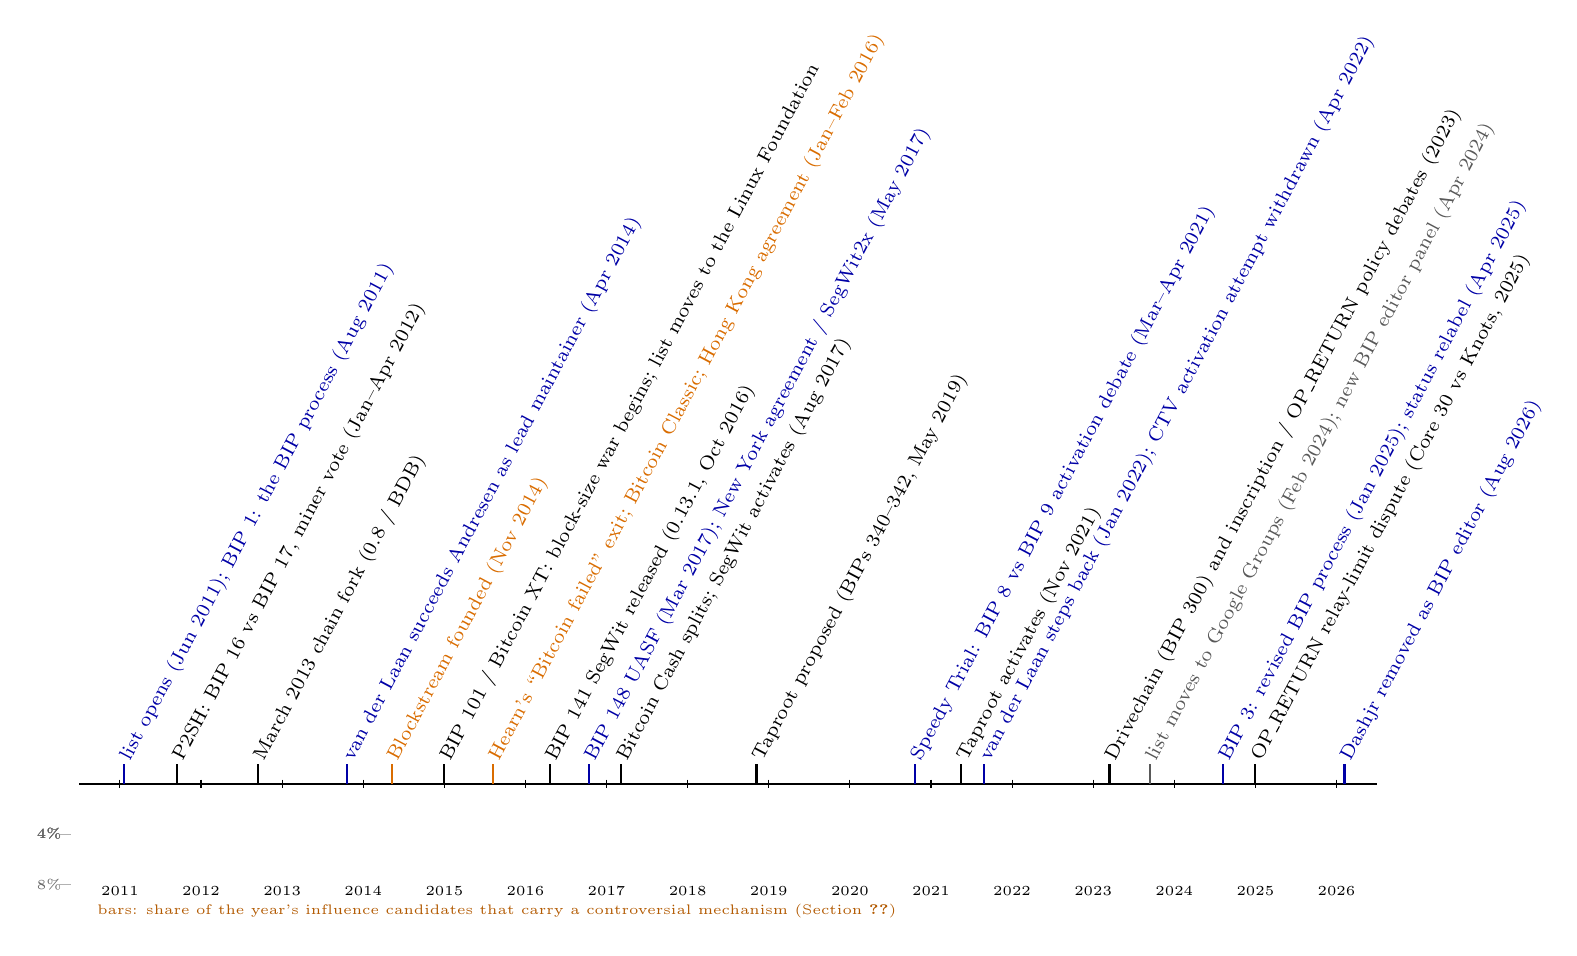
\begin{tikzpicture}[x=1.03cm, y=1cm, font=\scriptsize]
  % ---- yearly share of influence candidates carrying a controversial mechanism (filled by the assembly script) ----
  \foreach \yr/\p in {%%CONTRO_YEARS%%} {
    \pgfmathsetmacro{\xl}{\yr-2011+0.12}
    \pgfmathsetmacro{\xr}{\yr-2011+0.88}
    \pgfmathsetmacro{\h}{-\p*0.16}
    \fill[orange!25] (\xl,0) rectangle (\xr,\h);
  }
  \draw[gray!60] (-0.25,-0.64) -- (-0.1,-0.64) node[left, text=gray!80!black, font=\tiny] {4\%};
  \draw[gray!60] (-0.25,-1.28) -- (-0.1,-1.28) node[left, text=gray!80!black, font=\tiny] {8\%};
  \node[anchor=west, text=orange!70!black, font=\tiny] at (0.1,-1.62) {bars: share of the year's influence candidates that carry a controversial mechanism (Section~\ref{sec:rq6})};
  % ---- axis and years ----
  \draw[thick] (0,0) -- (16,0);
  \foreach \yr in {2011,2012,...,2026} {
    \draw (\yr-2011+0.5,0.05) -- (\yr-2011+0.5,-0.05);
    \node[font=\tiny] at (\yr-2011+0.5,-1.36) {\yr};
  }
  \tikzset{gov/.style={blue!65!black}, lang/.style={black}, venue/.style={gray!70!black}, corp/.style={orange!85!black}}
  \foreach \x/\c/\t in {
    2011.55/gov/{list opens (Jun 2011); BIP 1: the BIP process (Aug 2011)},
    2012.2/lang/{P2SH: BIP 16 vs BIP 17, miner vote (Jan--Apr 2012)},
    2013.2/lang/{March 2013 chain fork (0.8 / BDB)},
    2014.3/gov/{van der Laan succeeds Andresen as lead maintainer (Apr 2014)},
    2014.85/corp/{Blockstream founded (Nov 2014)},
    2015.5/lang/{BIP 101 / Bitcoin XT: block-size war begins; list moves to the Linux Foundation},
    2016.1/corp/{Hearn's ``Bitcoin failed'' exit; Bitcoin Classic; Hong Kong agreement (Jan--Feb 2016)},
    2016.8/lang/{BIP 141 SegWit released (0.13.1, Oct 2016)},
    2017.28/gov/{BIP 148 UASF (Mar 2017); New York agreement / SegWit2x (May 2017)},
    2017.68/lang/{Bitcoin Cash splits; SegWit activates (Aug 2017)},
    2019.35/lang/{Taproot proposed (BIPs 340--342, May 2019)},
    2021.3/gov/{Speedy Trial: BIP 8 vs BIP 9 activation debate (Mar--Apr 2021)},
    2021.87/lang/{Taproot activates (Nov 2021)},
    2022.15/gov/{van der Laan steps back (Jan 2022); CTV activation attempt withdrawn (Apr 2022)},
    2023.7/lang/{Drivechain (BIP 300) and inscription / OP\_RETURN policy debates (2023)},
    2024.2/venue/{list moves to Google Groups (Feb 2024); new BIP editor panel (Apr 2024)},
    2025.1/gov/{BIP 3: revised BIP process (Jan 2025); status relabel (Apr 2025)},
    2025.5/lang/{OP\_RETURN relay-limit dispute (Core 30 vs Knots, 2025)},
    2026.6/gov/{Dashjr removed as BIP editor (Aug 2026)}} {
    \draw[\c, thick] (\x-2011,0) -- (\x-2011,0.25);
    \node[\c, rotate=62, anchor=west, inner sep=1pt] at (\x-2011,0.27) {\t};
  }
\end{tikzpicture}
\caption{Landmark influences on the Bitcoin project from the start of the corpus (June 2011) to September 2026, above a corpus-derived measure of contestation: the share of each year's influence candidates that carry one of the seven controversial mechanisms (Section~\ref{sec:rq6}). Blue: governance and process; black: protocol decisions; orange: employer, funding and corporate stakes; grey: venues. Dates from the BIP repository, the reference implementation's history and the list itself.}
\label{fig:timeline}
\Description{A horizontal timeline from 2011 to 2026 with colour-coded events rising from the axis at an angle and a bar chart below the axis showing the yearly percentage of controversial influence candidates.}
\end{figure*}
